\section{A bit traveling through a lossless transmission line}
%In this section, the numerical analysis of a bit traveling through a lossless transmission line is %established ({\bf Figure CIRCUIT}). To this end, a rough analytical estimation of the simulation is %made

\subsection{General behavior of a bit traveling through a transmission line}
This section aims to predict, and thus validate, the behavior of the numerical simulation of the voltage in a LTL. A rough analytical approach is used, since it gives more insight in the physical nature of the problem. \\

Rearranging the telegrapher's equations for a LTL yields

\begin{equation}
\frac{\partial^2\hat{v}(z, t)}{\partial z^2} - k^2\frac{\partial^2 \hat{v}(z, t)}{\partial t^2} = 0, \quad k = \frac{1}{c}= \sqrt{LC} = \mathrm{cte}.
\label{tele}
\end{equation}

This is know as the wave equation. This means that the solution of (\ref{tele}) is a superposition of two voltage waves traveling in opposite directions. That is,

\begin{equation}
\hat{v}(z, t) = \underbrace{\hat{v}^{+}(z - ct)}_{\text{forward wave}} + \underbrace{\hat{v}^{-}(z + ct)}_{\text{backward wave}}.
\end{equation}

If one assumes that at $t < 0$ no voltages are present in the TL, and at $t=0$ the generator $\hat{e}_g$ is excited, a forward wave $\hat{v}^{+}$ is produced and traveling with constant speed $c = \frac{1}{\sqrt{LC}}$ through the TL towards te load. Since the line is lossless, its amplitude $|\hat{v}| = |\hat{v}^{+}|$ remains constant. When the voltage wave arrives at the load i.e. when $t = \frac{d}{c}$, it is partially absorbed and reflected; the forward wave becomes a backward wave with a lower amplitude. At $t = \frac{2d}{c}$ the backward wave arrives at the generator and is again reflected with a decreased amplitude. This process goes on until the amplitude is fully dampened and no voltage waves exist in the TL.

\begin{figure*}
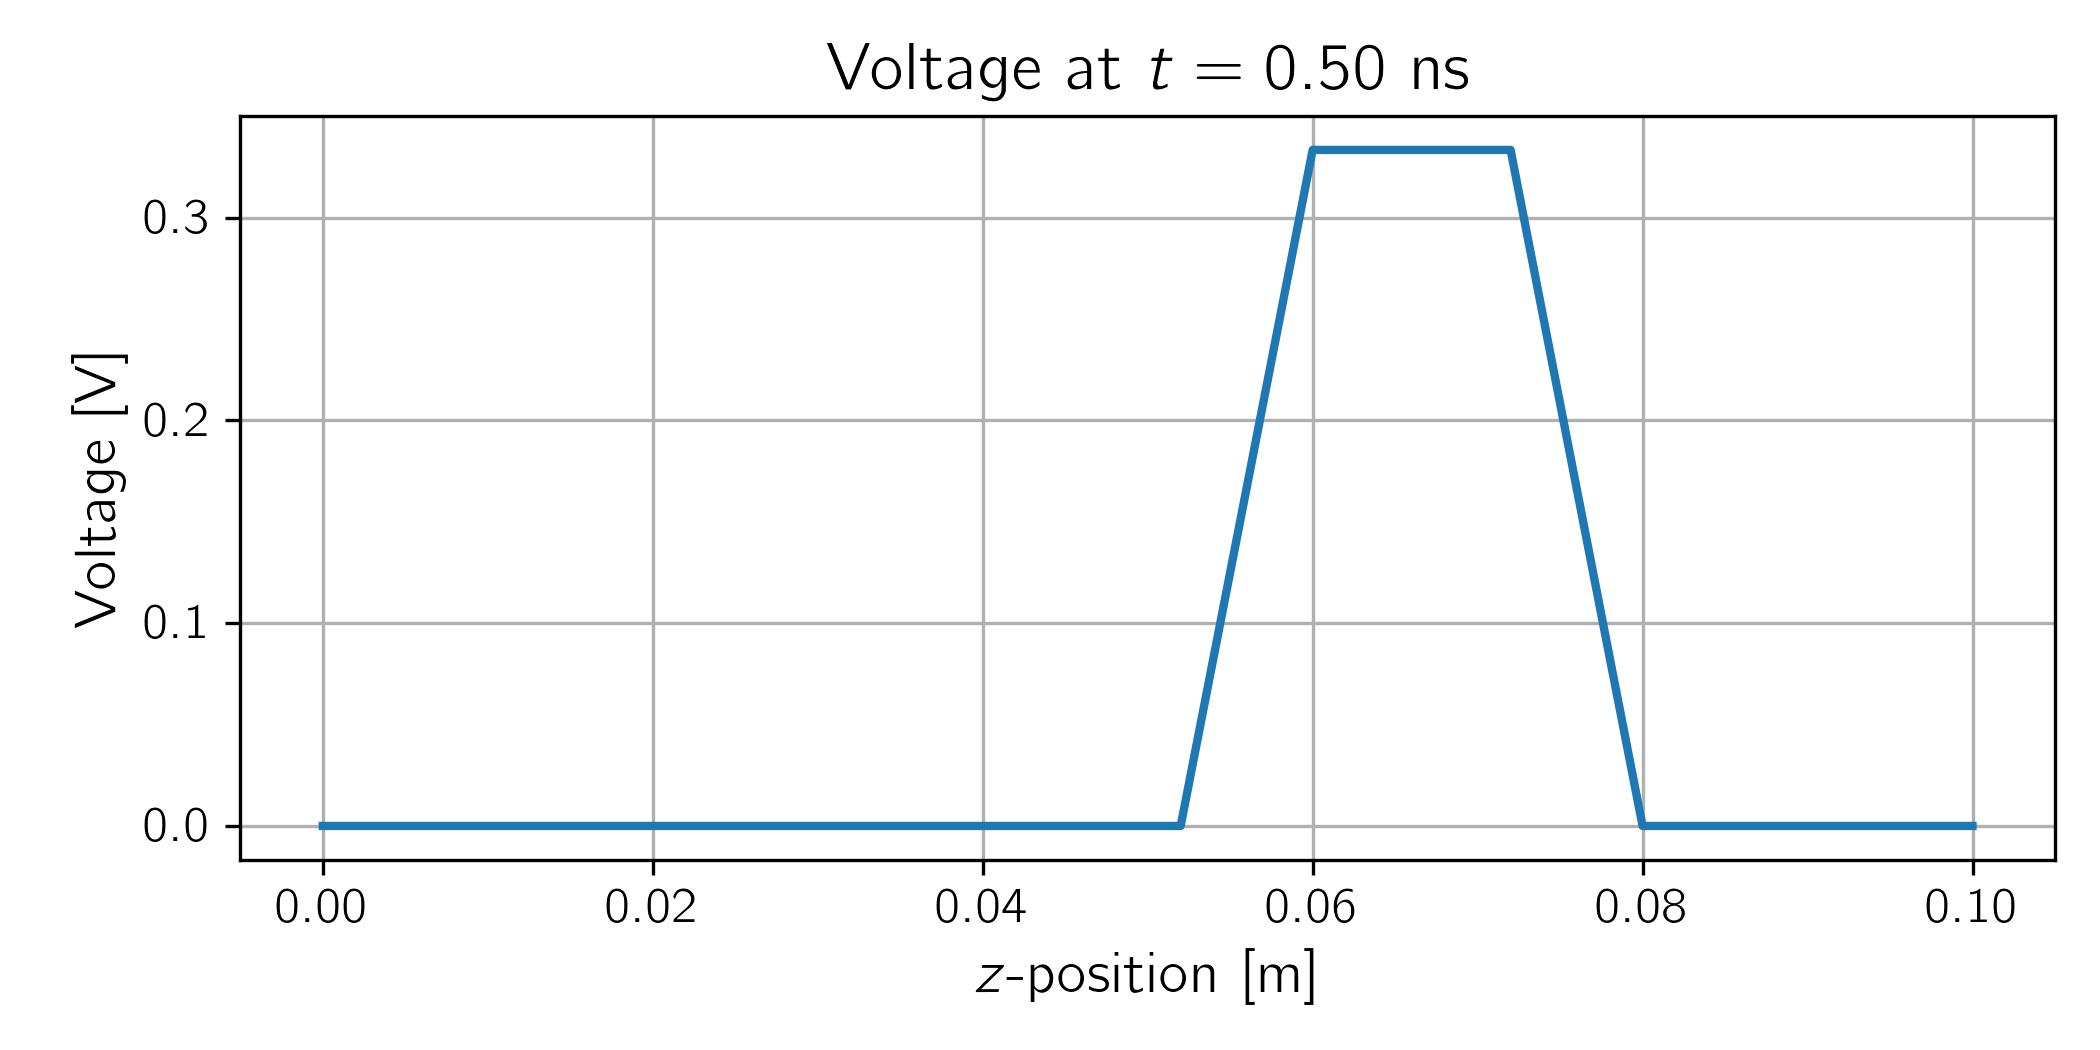
\includegraphics[width = 0.5\linewidth]{exampleposition.png}
\end{figure}
